\documentclass{beamer}
\usetheme{Warsaw}

\usepackage{graphicx} % Allows including images
\usepackage{booktabs} % Allows the use of \toprule, \midrule and \bottomrule in tables
\usepackage{listings}
\usepackage[utf8]{inputenc}
\usepackage[overlay,absolute]{textpos}
\usepackage[]{algorithm2e}
\usepackage{amssymb}
\usepackage{tikz}
\usetikzlibrary{arrows, automata}

\AtBeginSection[]
{
\begin{frame}<beamer>
\frametitle{Plan}
\footnotesize{
\tableofcontents[
  currentsection,
  hideothersubsections
]
}
\end{frame}
}

\lstset{language=C++,
                basicstyle=\ttfamily,
                keywordstyle=\color{green}\ttfamily,
                stringstyle=\color{red}\ttfamily,
                commentstyle=\color{cyan}\ttfamily,
                morecomment=[l][\color{cyan}]{\#},
                escapechar=@
}

\setbeamercolor{normal text}{fg=white,bg=black!90}
\setbeamercolor{structure}{fg=white}

\setbeamercolor{alerted text}{fg=red!85!black}

\setbeamercolor{item projected}{use=item,fg=black,bg=item.fg!35}

\setbeamercolor*{palette primary}{use=structure,fg=structure.fg}
\setbeamercolor*{palette secondary}{use=structure,fg=structure.fg!95!black}
\setbeamercolor*{palette tertiary}{use=structure,fg=structure.fg!90!black}
\setbeamercolor*{palette quaternary}{use=structure,fg=structure.fg!95!black,bg=black!80}

\setbeamercolor*{framesubtitle}{fg=white}

\setbeamercolor*{block title}{parent=structure,bg=black!60}
\setbeamercolor*{block body}{fg=black,bg=black!10}
\setbeamercolor*{block title alerted}{parent=alerted text,bg=black!15}
\setbeamercolor*{block title example}{parent=example text,bg=black!15}

\author[Félix-Antoine Ouellet]{Félix-Antoine Ouellet}

\title[PolyOpt\hspace{2em}\insertframenumber/\inserttotalframenumber]{Compilation polyhédrale}

\institute{Université de Sherbrooke}

\date{4 décembre 2014}

\begin{document}

\begin{frame}
\titlepage % Print the title page as the first slide
\end{frame}

\begin{frame}
\tableofcontents[hideallsubsections]
\end{frame}

\section{Motivation}
\begin{frame}
\frametitle{L'ère du parallélisme}
\begin{center}
\colorbox{white}{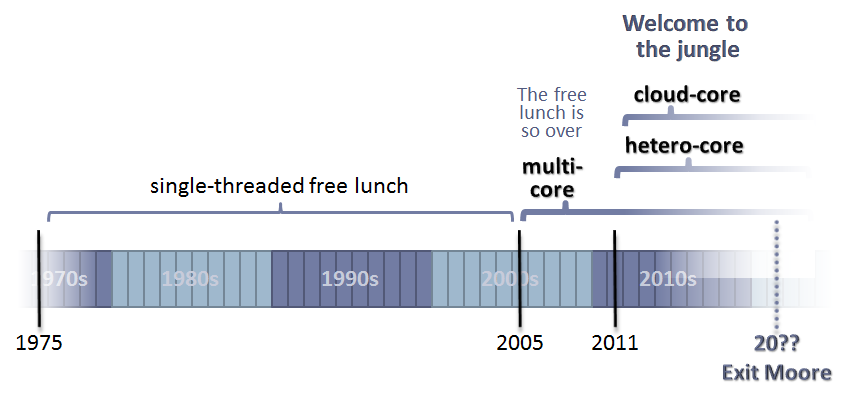
\includegraphics[scale=0.48]{parallel.png}}
\end{center}
\end{frame}

\begin{frame}
\frametitle{Problèmes courants}
\framesubtitle{Rendre le parallélisme accessible}
On cherche toujours les meilleures abstractions pour le calcul parallèle
\begin{itemize}
\item \textit{Threads}
\item Tâches
\item Langages dédiés
\item Parallélisme implicite
\end{itemize}
\end{frame}

\begin{frame}
\frametitle{Problèmes courants}
\framesubtitle{Parallélisation d'applications existantes}
Comment améliorer la performance de \textit{legacy code}?
\begin{itemize}
\item Mettre tout à terre et recommencer
\item Payer des développeurs pour améliorer des sections critiques
\item Espérer qu'un outil améliore magiquement la situation
\end{itemize}
\end{frame}

\begin{frame}
\frametitle{Problèmes courants}
\framesubtitle{Compilateurs}
Les compilateurs modernes ont beaucoup de difficulté à extraire du parallélisme d'applications écrites de façon séquentielles
\begin{itemize}
\item Problèmes théoriques très difficile à résoudre
\item Aucun succès majeur jusqu'à maintenant
\item Les compilateurs modernes manquent d'outils pour la tâche
\end{itemize}
\end{frame}

\section{Compilation traditionnelle}
\subsection{Bases de la compilation}
\begin{frame}
\frametitle{Notions importantes}
\begin{itemize}
\item Transforme un programme écrit dans un langage (de haut niveau) en un programme écrit dans un autre langage (de bas niveau).
\item Maintient la sémantique du programme original.
\end{itemize}
\end{frame}

\begin{frame}
\frametitle{Architecture usuelle}
\begin{center}
\begin{tikzpicture}[-,>=stealth',shorten >=1pt,auto,node distance=4.5cm,
thick,main node/.style={rectangle,draw,font=\sffamily\Large\bfseries}]
\draw[white] (0, 0) rectangle (2, 3);
\draw[white] (2, 0) rectangle (4, 3);
\draw[white] (4, 0) rectangle (6, 3);
\node[draw=none] (1) at (1, 1.5) {\textit{Frontend}};
\node[draw=none] (2) at (3, 1.5) {\textit{Optimizer}};
\node[draw=none] (3) at (5, 1.5) {\textit{Backend}};
\node[draw=none] (4) at (-1.5, 1.5) {Code source};
\node[draw=none] (5) at (7.5, 1.5) {Code machine};
\end{tikzpicture}
\end{center}
\begin{textblock}{6}(4, 9.6)
$\rightarrow$
\end{textblock}
\begin{textblock}{6}(12, 9.6)
$\rightarrow$
\end{textblock}
\end{frame}

\subsection{Processus de compilation}
\begin{frame}
\frametitle{Étape 1 - \textit{Frontend}}
\begin{itemize}
\item \textit{Lexing}
\item \textit{Parsing}
\item Analyse sémantique
\item Travaille sur le code et sur un AST
\end{itemize}
\end{frame}

\begin{frame}[fragile]
\frametitle{Étape 1 - \textit{Frontend}}
\framesubtitle{AST}
\begin{columns}
\begin{column}{0.5\textwidth}
\footnotesize{
\begin{lstlisting}
int countOdd(int A[],
             int N) {
  int cpt = 0;
  for (int i = 0; i < N;
  ++i)
    if (A[i] % 2 == 1)
      cpt++;
  return cpt;
}
\end{lstlisting}}
\end{column}
\begin{column}{0.5\textwidth}
\colorbox{white}{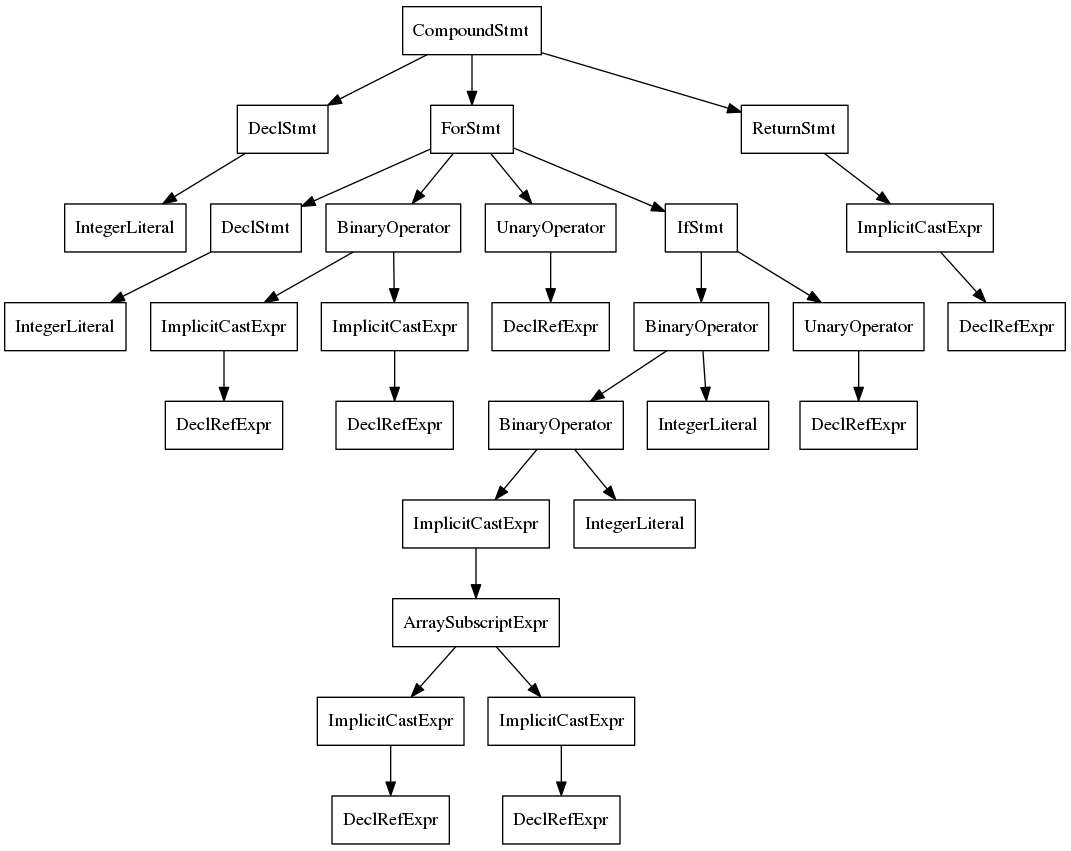
\includegraphics[scale=0.15]{AST.png}}
\end{column}
\end{columns}
\begin{textblock}{6}(7.1, 9)
\Huge{$\Rightarrow$}
\end{textblock}
\end{frame}

\begin{frame}
\frametitle{Étape 2 - Optimisateur}
\begin{itemize}
\item Analyse le flot des données
\item Optimisations indépendantes de la machine
\item Travaille sur un CFG
\end{itemize}
\end{frame}

\begin{frame}
\frametitle{Étape 2 - Optimisateur}
\framesubtitle{CFG}
\begin{columns}
\begin{column}{0.5\textwidth}
\colorbox{white}{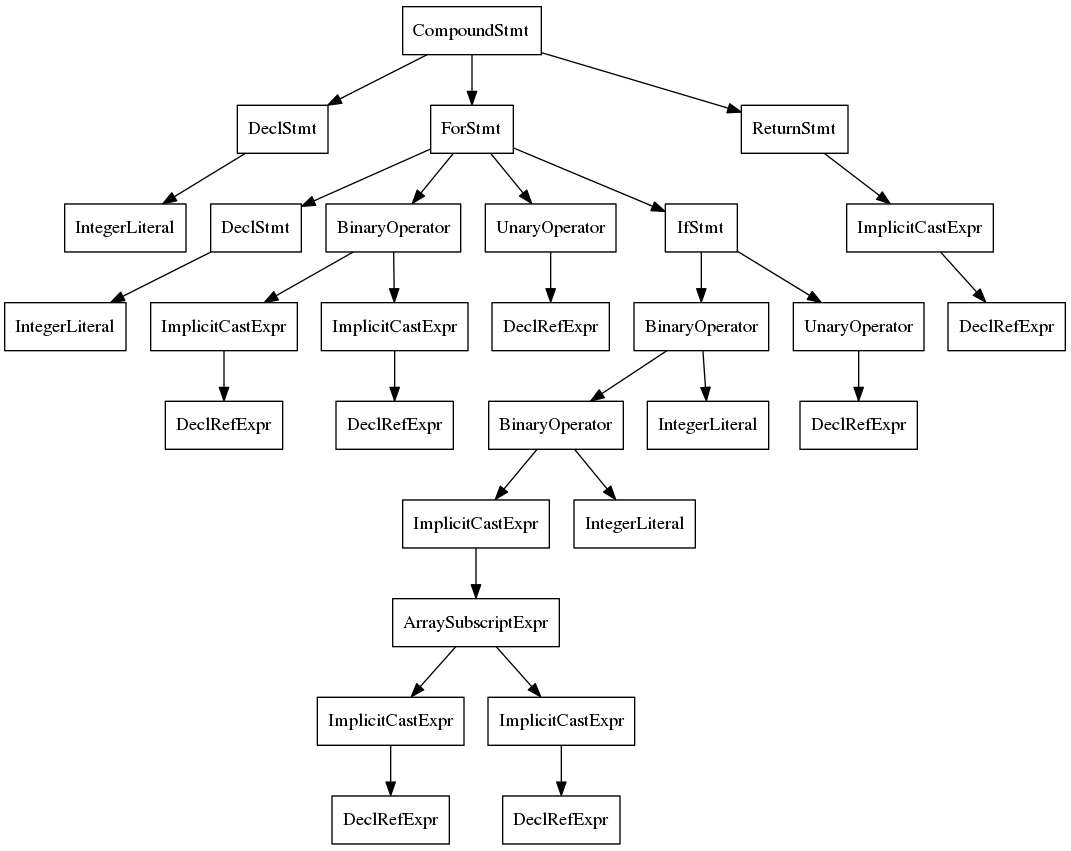
\includegraphics[scale=0.15]{AST.png}}
\end{column}
\begin{column}{0.5\textwidth}
\begin{center}
\colorbox{white}{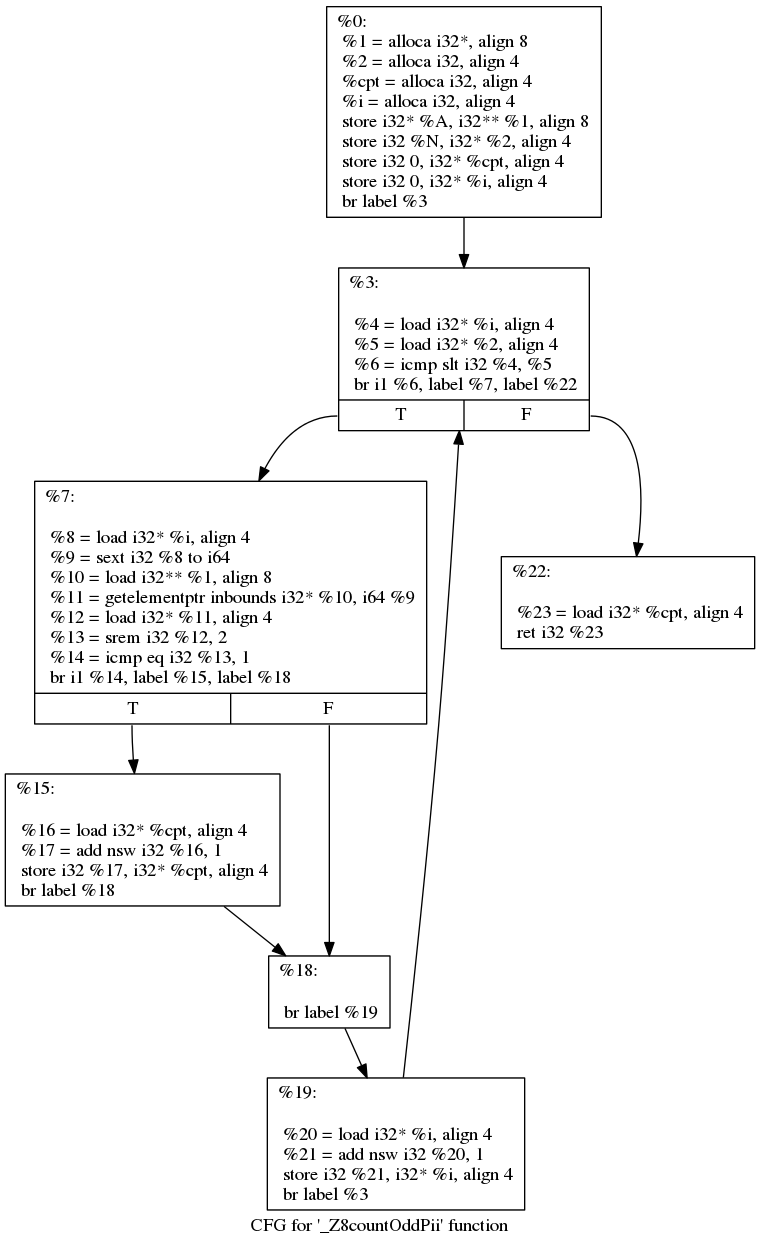
\includegraphics[scale=0.13]{cfg.png}}
\end{center}
\end{column}
\end{columns}
\begin{textblock}{6}(8.35, 9)
\Huge{$\Rightarrow$}
\end{textblock}
\end{frame}

\begin{frame}
\frametitle{Étape 3 - \textit{Backend}}
\begin{itemize}
\item Optimisations spécifiques à la machine
\item Génére le code machine
\item Travaille sur un CFG
\end{itemize}
\end{frame}

\subsection{Représentation intermédiaire}
\begin{frame}
\frametitle{Représentation intermédiaire}
\framesubtitle{Illustration}
\begin{center}
\colorbox{white}{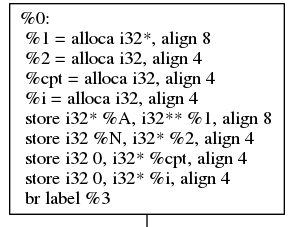
\includegraphics[scale=0.7]{basic block.png}}
\end{center}
\end{frame}

\begin{frame}
\frametitle{Représentation intermédiaire}
\framesubtitle{Forme SSA}
\begin{itemize}
\item Chaque variable est affectée une seule fois
\item Chaque variable est définie avant d'être utilisée
\item Une variable dans un programme est représentée par plusieurs variables en forme SSA
\end{itemize}
\end{frame}

\begin{frame}
\frametitle{Représentation intermédiaire}
\framesubtitle{Avantages}
\begin{itemize}
\item Simplifie et améliore les analyses de flot de données
\item Simplifie et améliore les optimisations indépendantes de la machine
\item Permet de vérifier plus facilement les transformations effectuées
\end{itemize}
\end{frame}

\begin{frame}
\frametitle{Représentation intermédiaire}
\framesubtitle{Limitations}
\begin{itemize}
\item Requiert des extensions pour bien optimiser les boucles
\item Ne permet pas d'effectuer plusieurs transformations de boucles simultanément
\item Requiert des extensions pour gérer le parallélisme
\end{itemize}
\end{frame}

\section{Approche polyhédrale}
\subsection{Représentation}
\begin{frame}
\frametitle{Cible}
L'optimisation polyhédrale touche les parties à controle statique (SCoP) d'un programme
\end{frame}

\begin{frame}
\frametitle{SCoP}
\framesubtitle{Définition}
\begin{itemize}
\item Ensemble d'énoncés dans une boucle
\item Boucle dont les bornes sont des fonctions affines des itérateurs et paramètres avoisinants
\item Accès mémoire doivent être des fonctions affines des itérateurs et paramètres avoisinants
\end{itemize}
\end{frame}

\begin{frame}[fragile]
\frametitle{SCoP}
\framesubtitle{Exemple}
\begin{lstlisting}
for (int i = 0; i < 32; ++i)
  for (int j = 0; j < 1000; ++j)
    A[i][j] += 10;
\end{lstlisting}
\end{frame}

\begin{frame}[fragile]
\frametitle{Représentation polyhédrale}
\framesubtitle{Composantes}
Une représentation polyhédrale doit pouvoir encapsuler toutes les informations concernant:
\begin{itemize}
\item Le domaine de chaque énoncé
\item L'ordre d'exécution de chaque instances de chaque énoncé
\item Les accès mémoire effectuées par chaque énoncé
\end{itemize}
\end{frame}

\begin{frame}[fragile]
\frametitle{Représentation polyhédrale}
\framesubtitle{Exemple}
\begin{lstlisting}
for (int i = 0; i < 32; ++i)
  for (int j = 0; j < 1000; ++j)
    A[i][j] += 10; // Stmt1
\end{lstlisting}
\vspace{0.75cm}
$D_{Stmt1} = \{Stmt1[i,j]: 0 \leq i < 32 \wedge 0 \leq j < 1000 \}$\\
$S_{Stmt1} = \{Stmt1[i,j] \rightarrow [i,j] \}$\\
$A_{Stmt1} = \{Stmt1[i,j] \rightarrow A[i,j] \}$\\
\end{frame}

\begin{frame}[fragile]
\frametitle{Représentation polyhédrale}
\framesubtitle{Illustration}
\begin{lstlisting}
for (int i = 0; i < 32; ++i)
  for (int j = 0; j < 1000; ++j)
    A[i][j] += 10; // Stmt1
\end{lstlisting}
\vspace{-0.5cm}
\begin{center}
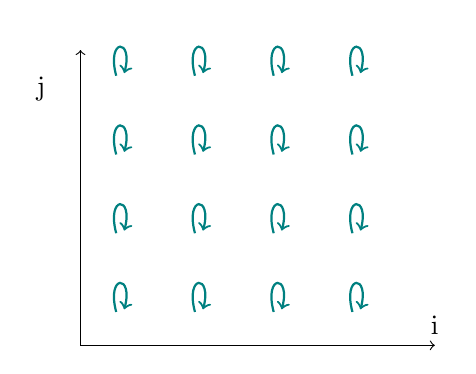
\begin{tikzpicture}
   \tikzstyle{place}=[circle,thick,draw=white,fill=white,minimum size=0.1mm]
   \node[place] (1) {};
   \node[place] (2) [right of=1] {};
   \node[place] (3) [right of=2] {};
   \node[place] (4) [right of=3] {};
   \node[place] (5) [below of=1] {};
   \node[place] (6) [right of=5] {};
   \node[place] (7) [right of=6] {};
   \node[place] (8) [right of=7] {};
   \node[place] (9) [below of=5] {};
   \node[place] (10) [right of=9] {};
   \node[place] (11) [right of=10] {};
   \node[place] (12) [right of=11] {};
   \node[place] (13) [below of=9] {};
   \node[place] (14) [right of=13] {};
   \node[place] (15) [right of=14] {};
   \node[place] (16) [right of=15] {};
   
   \node (17) [left of=1] {j};
   \node (18) [right of=16] {i};
   
   \path[teal, thick, ->] (1)  edge  [loop above] node {} ();
   \path[teal, thick, ->] (2)  edge  [loop above] node {} ();
   \path[teal, thick, ->] (3)  edge  [loop above] node {} ();
   \path[teal, thick, ->] (4)  edge  [loop above] node {} ();
   \path[teal, thick, ->] (5)  edge  [loop above] node {} ();
   \path[teal, thick, ->] (6)  edge  [loop above] node {} ();
   \path[teal, thick, ->] (7)  edge  [loop above] node {} ();
   \path[teal, thick, ->] (8)  edge  [loop above] node {} ();
   \path[teal, thick, ->] (9)  edge  [loop above] node {} ();
   \path[teal, thick, ->] (10) edge  [loop above] node {} ();
   \path[teal, thick, ->] (11) edge  [loop above] node {} ();
   \path[teal, thick, ->] (12) edge  [loop above] node {} ();
   \path[teal, thick, ->] (13) edge  [loop above] node {} ();
   \path[teal, thick, ->] (14) edge  [loop above] node {} ();
   \path[teal, thick, ->] (15) edge  [loop above] node {} ();
   \path[teal, thick, ->] (16) edge  [loop above] node {} ();
   
   \draw[->] (-0.5,-3.25) -- (-0.5,0.5);
   \draw[->] (-0.5,-3.25) -- (4,-3.25);
\end{tikzpicture}
\end{center}
\end{frame}

\subsection{Transformations}
\begin{frame}
\frametitle{Transformations}
\begin{itemize}
\item Une transformation consiste à appliquer une opération algébrique sur l'ordre d'exécution du \textit{SCoP} traité
\item Plusieurs transformations peuvent être effectuée en un seul calcul
\end{itemize}
\end{frame}

\begin{frame}[fragile]
\frametitle{Transformations}
\frametitle{Exemple - Partie 1}
$T_{Interchange} = \{[i,j] \rightarrow [j,i] \}$\\
\vspace{0.5cm}
$D_{Stmt1} = \{Stmt1[i,j]: 0 \leq i < 32 \wedge 0 \leq j < 1000 \}$\\
$S'_{Stmt1} = S \circ T_{Interchange}$\\
$A_{Stmt1} = \{Stmt1[i,j] \rightarrow A[i,j] \}$\\
\vspace{0.5cm}
\begin{lstlisting}
for (int j = 0; j < 1000; ++j)
  for (int i = 0; i < 32; ++i)
    A[i][j] += 10; // Stmt1
\end{lstlisting}
\end{frame}

\begin{frame}[fragile]
\frametitle{Transformations}
\frametitle{Exemple - Partie 2}
$T_{Interchange} = \{[i,j] \rightarrow [j,i] \}$\\
$T_{StripMine} = \{[i,j] \rightarrow [i,jj,j]: jj \mod 4 = 0 \wedge jj \leq j < jj + 4 \}$\\
\vspace{0.5cm}
$D_{Stmt1} = \{Stmt1[i,j]: 0 \leq i < 32 \wedge 0 \leq j < 1000 \}$\\
$S'_{Stmt1} = S \circ T_{Interchange} \circ T_{StripMine}$\\
$A_{Stmt1} = \{Stmt1[i,j] \rightarrow A[i,j] \}$\\
\vspace{0.5cm}
\begin{lstlisting}
for (int j = 0; j < 1000; ++j)
  for (int ii = 0; ii < 32; ii += 4)
    for (int i = ii; i < ii+4; ++i)
      A[i][j] += 10; // Stmt1
\end{lstlisting}
\end{frame}

\subsection{Limitations}
\begin{frame}
\frametitle{Limitations}
\begin{itemize}
\item Accès non affines
\item Boucles irrégulières
\item Pointeurs
\end{itemize}
\end{frame}

\section{Parallélisation automatique}
\subsection{Intuition}
\begin{frame}
\frametitle{Intuition}
\begin{itemize}
\item Le modèle polyhédral travaille sur les instances des énoncés
\item<2-> Chaque instance peut être considéré comme une tâche
\item<3-> Il suffit donc de trouver un plan d'exécution de ces tâches
\end{itemize}
\end{frame}

\begin{frame}
\frametitle{Intuition}
\framesubtitle{Illustration}
\begin{textblock}{6}(1, 6)
\begin{center}
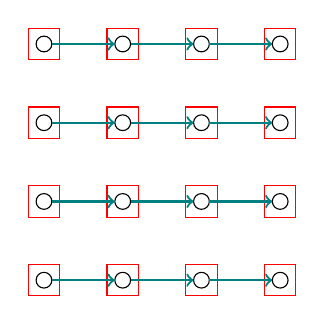
\begin{tikzpicture}
    \foreach \x in {0,1,2,3}
    \foreach \y in {0,1,2,3}
    {
    \draw[fill=white] (\x,\y) circle (0.1cm);
    \draw[red] (\x-0.2,\y-0.2) rectangle (\x+0.2,\y+0.2);
    }
    \foreach \x in {0,1,2}
    \foreach \y in {0,1,2,3}
    {
    \draw[thick, ->, teal] (\x+0.1,\y) -- (\x+0.9,\y);
    }
\end{tikzpicture}
\end{center}
\end{textblock}

\begin{textblock}{6}(5, 8)
\begin{center}
\Huge{$\rightarrow$}
\end{center}
\end{textblock}

\begin{textblock}{6}(9, 6)
\begin{center}
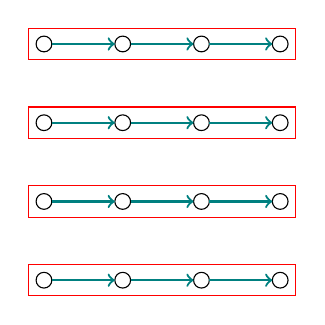
\begin{tikzpicture}
    \foreach \x in {0,1,2,3}
    \foreach \y in {0,1,2,3}
    {
    \draw[fill=white] (\x,\y) circle (0.1cm);
    }
    \foreach \x in {0,1,2}
    \foreach \y in {0,1,2,3}
    {
    \draw[thick, ->, teal] (\x+0.1,\y) -- (\x+0.9,\y);
    }
    \foreach \y in {0,1,2,3}
    {
    \draw[red] (-0.2,\y-0.2) rectangle (3.2,\y+0.2);
    }
\end{tikzpicture}
\end{center}
\end{textblock}
\end{frame}

\subsection{Pratique}
\begin{frame}
\frametitle{Rappel}
Une boucle peut être parallélisée si elle ne contient pas de dépendences mémoire portées par la boucle
\end{frame}

\begin{frame}[fragile]
\frametitle{Rappel}
\begin{lstlisting}
for (int i = 0; i < N; ++i) {
  A[i] = B[i] + C[i];
  D[i] = A[i] + 10;
}

for (int i = 0; i < N; ++i) {
  A[i+1] = A[i] + B[i];
}
\end{lstlisting}
\begin{textblock}{6}(13, 7)
	\Huge{\checkmark}
\end{textblock}
\begin{textblock}{6}(13, 10.75)
	\Huge{X}
\end{textblock}
\end{frame}

\begin{frame}
\frametitle{Dépendences dans le modèle polyhédral}
Pour obtenir les dépendences dans une boucle, il faut:
\begin{itemize}
\item Séparer les accès en écriture des accès en lecture
\item Trouver l'intersection de ces ensembles d'accès
\item Obtenir la distance entre ces accès
\end{itemize}
\end{frame}

\begin{frame}[fragile]
\frametitle{Dépendences dans le modèle polyhédral}
\framesubtitle{Séparer les accès en écriture des accès en lecture}
\begin{lstlisting}
for (int i = 0; i < 100; ++i) {
  A[i] = B[i] + C[i]; // Stmt1
  D[i] = A[i] + 10;   // Stmt2
}
\end{lstlisting}
$A_{Stmt1_W} = \{Stmt1[i] \rightarrow A[i] \}$\\
$A_{Stmt1_R} = \{Stmt1[i] \rightarrow \emptyset \}$\\
\vspace{0.2cm}
$A_{Stmt2_W} = \{Stmt2[i] \rightarrow \emptyset \}$\\
$A_{Stmt2_R} = \{Stmt2[i] \rightarrow A[i] \}$\\
\end{frame}

\begin{frame}[fragile]
\frametitle{Dépendences dans le modèle polyhédral}
\framesubtitle{Trouver l'intersection de ces ensembles d'accès}
\begin{lstlisting}
for (int i = 0; i < 100; ++i) {
  A[i] = B[i] + C[i]; // Stmt1
  D[i] = A[i] + 10;   // Stmt2
}
\end{lstlisting}
$A_{Stmt1_W} \cap A_{Stmt1_R} = \emptyset $\\
$A_{Stmt1_W} \cap A_{Stmt2_R} = A[i] $\\
$A_{Stmt2_W} \cap A_{Stmt1_R} = \emptyset $\\
$A_{Stmt2_W} \cap A_{Stmt2_R} = \emptyset $\\
\end{frame}

\begin{frame}[fragile]
\frametitle{Dépendences dans le modèle polyhédral}
\framesubtitle{Obtenir la distance entre ces accès}
\begin{lstlisting}
for (int i = 0; i < 100; ++i) {
  A[i] = B[i] + C[i]; // Stmt1
  D[i] = A[i] + 10;   // Stmt2
}
\end{lstlisting}
$A_{Stmt1_W} = \{Stmt1[i] \rightarrow A[i] \}$\\
$A_{Stmt2_R} = \{Stmt2[i] \rightarrow A[i] \}$\\
\begin{textblock}{6}(8, 11)
\huge{$\rightarrow 0$}
\end{textblock}
\end{frame}

\begin{frame}[fragile]
\frametitle{Génération de code parallèle}
\begin{lstlisting}
#pragma omp parallel
for (int i = 0; i < 100; ++i) {
  A[i] = B[i] + C[i]; // Stmt1
  D[i] = A[i] + 10;   // Stmt2
}
\end{lstlisting}
\end{frame}

\section{État actuel}
\begin{frame}
\frametitle{Résultats obtenus}
\framesubtitle{Contexte}
\begin{itemize}
\item PolyBench
\item Clang -O3
\item Polly
\item Valeurs en virgule flottante avec double précision
\item Intel Xeon X5670 @ 2.93 GHz (12 coeurs, 24 \textit{threads})
\end{itemize}
\end{frame}

\begin{frame}
\frametitle{Résultats obtenus}
\framesubtitle{Séquentiel}
\begin{center}
\colorbox{white}{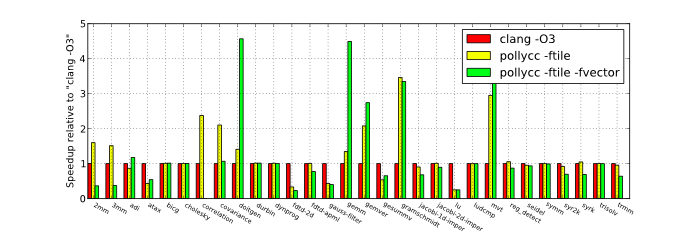
\includegraphics[scale=0.36]{sequential-small.png}}
\end{center}
\end{frame}

\begin{frame}
\frametitle{Résultats obtenus}
\framesubtitle{Parallèle}
\begin{center}
\colorbox{white}{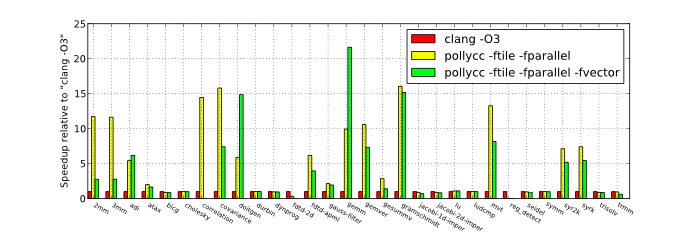
\includegraphics[scale=0.36]{parallel-small.png}}
\end{center}
\end{frame}

\begin{frame}
\frametitle{Support présent}
\begin{itemize}
\item LLVM (Polly)
\item GCC (Graphite)
\item Langages expérimentaux (X10)
\item Plateformes expérimentales (PLUTO)
\end{itemize}
\end{frame}

\section{Conclusion}
\begin{frame}
\frametitle{Conclusion}
\begin{itemize}
\item Offre une façon différente de raisonner sur l'optimisation de boucles et la parallélisation automatique
\item Représente possiblement la meilleure chance de produire du parallélisme implicite
\end{itemize}
\end{frame}

\end{document}